\chapter{Simple Storage Service (S3)}\label{ch:simple-storage-service}

\section{What is Simple Storage Service (S3)?}
AWS S3 is a form of cloud-based object storage.
This is a style of network filesystem that treats each file as a separate object with a unique ID, which allows each
object to be served individually over a network with a single URL, which can also be enhanced with a content delivery
network~\parencite{amazon2022cloud}.

Each S3 instance is seperated into logical containers known as buckets.
Each S3 bucket can have its own credentials, its own endpoint and other permissions and configuration.
Object storage is particularly useful when creating an application that scales as you are billed per unit of storage
that you use, and in theory are able to use infinite storage as your application demands.
The only limitation with object storage is how much you are able to pay for.
Each object is automatically replicated across many nodes, providing data redundancy against multiple different
availability zones.

S3 is perhaps the most popular AWS service and used by many SaaS applications across the internet, for instance
Instagram, Facebook, Discord and Twitter are all known for using S3 or S3-style storage.
The advent of object storage has created an almost de-facto standard, which has lead for the creation of many
'S3-compatible' or 'S3-like' competitor solutions, such as those run by Google Cloud and Microsoft Azure.

\begin{enumerate}
    \section{Creating an S3 Bucket}

        \item Setting up an encryption key to be managed by AWS was the most secure option.
            \begin{figure}[H]
                \centering
                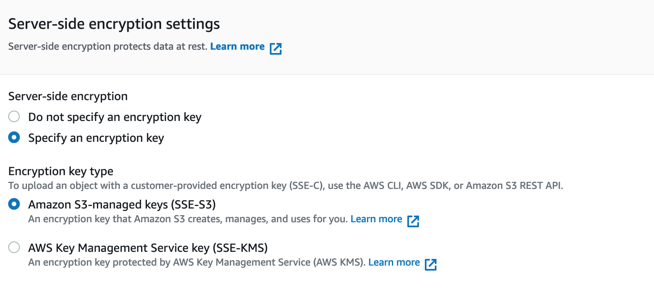
\includegraphics[width=\textwidth]{resources/s3/s3_encryption.PNG}
                \caption{Setting up S3 Encryption Key}
                \label{fig:s3-image-2}
            \end{figure}


    \item Enabling server-side encryption
        \begin{figure}[H]
            \centering
            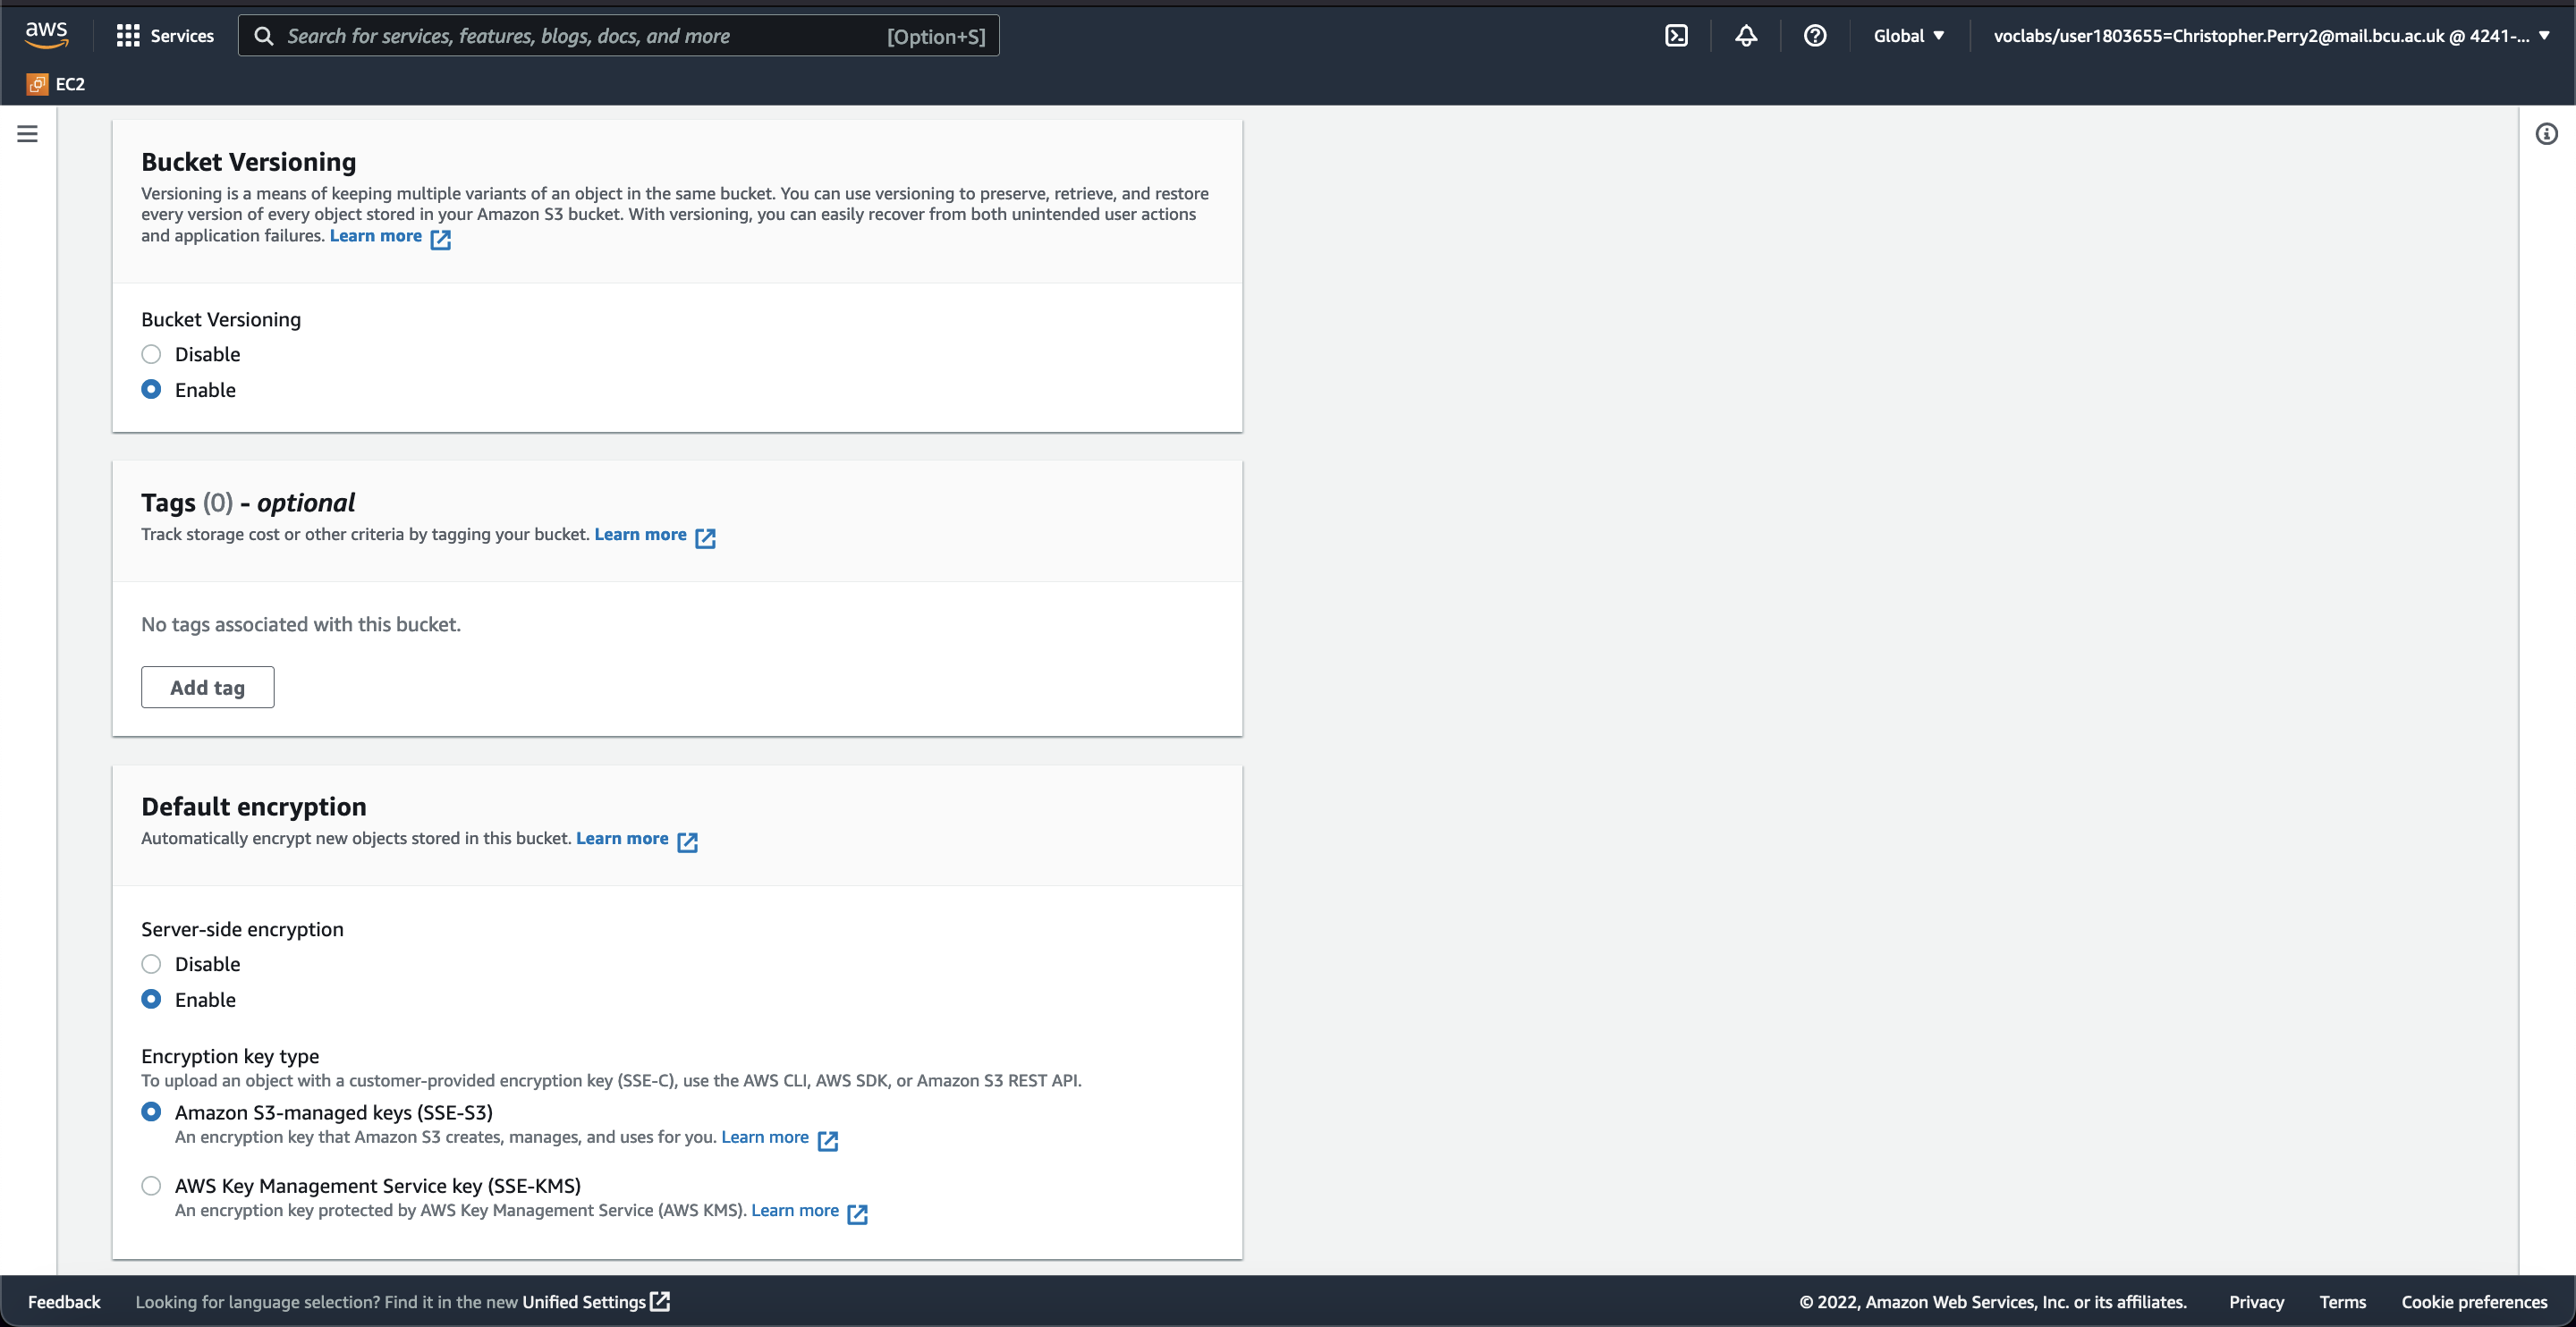
\includegraphics[width=\textwidth]{resources/s3/s3-versioning-encrypting.png}
            \caption{Setting up S3 Versioning and Encryption Settings}
            \label{fig:s3-versioning-encrypting}
        \end{figure}

    \item Setting object ownership used the recommended option as all of our images should be public, so fine-grain ACL control was not needed.
        \begin{figure}[H]
            \centering
            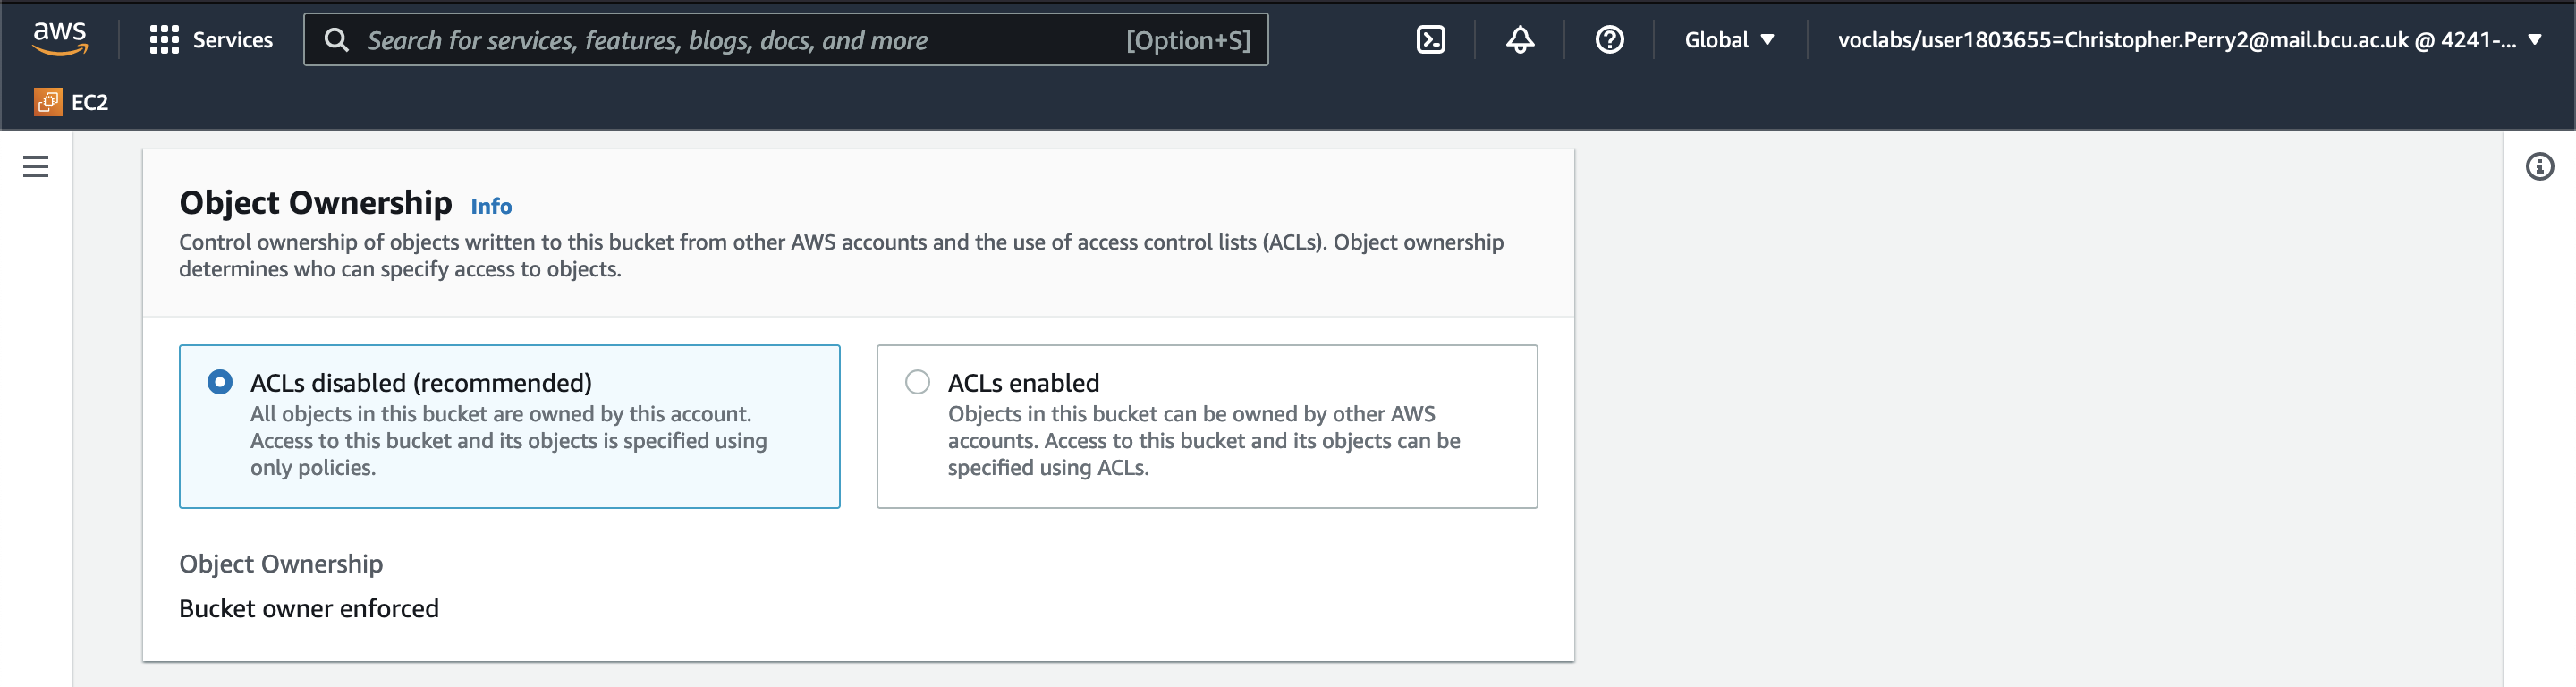
\includegraphics[width=\textwidth]{resources/s3/s3-object-ownership.png}
            \caption{Setting S3 Object Ownership}
            \label{fig:s3-object-ownership}
        \end{figure}


    \item Allowing public read access to the S3 bucket, as all of our images should be public static assets, no private assets are needed.
        \begin{figure}[H]
            \centering
            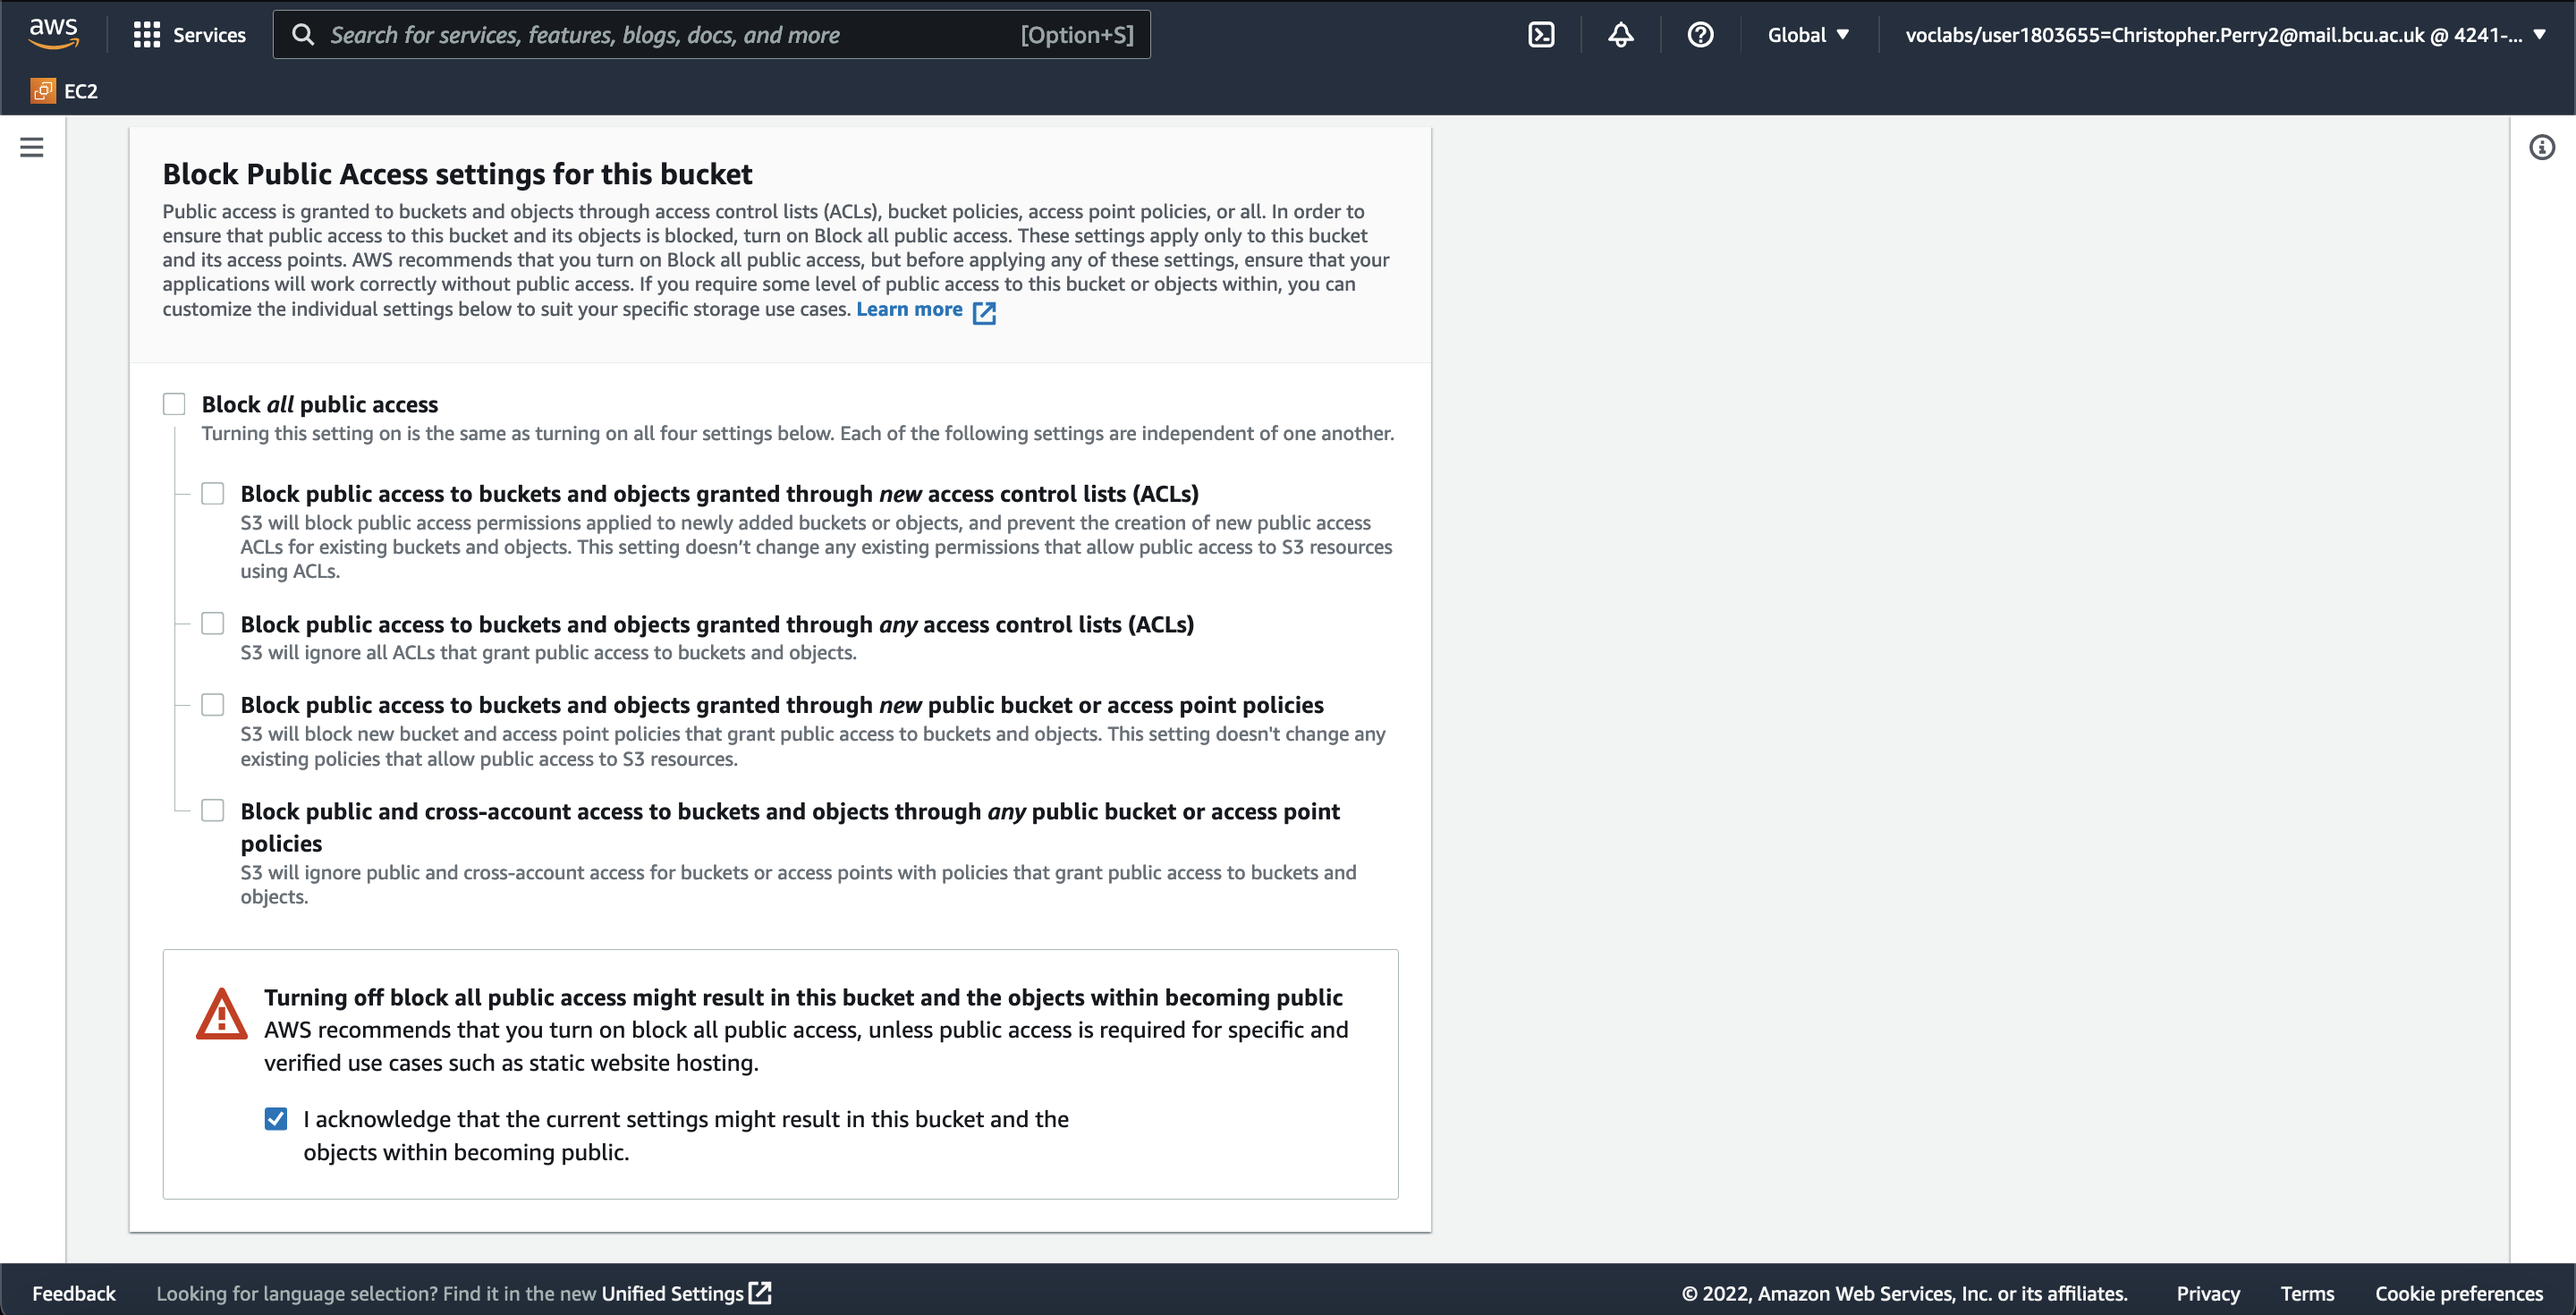
\includegraphics[width=\textwidth]{resources/s3/s3-public-access.png}
            \caption{Allowing Public Read Access}
            \label{fig:s3-public-access}
        \end{figure}


    \item S3 bucket has been created successfully.
        \begin{figure}[H]
            \centering
            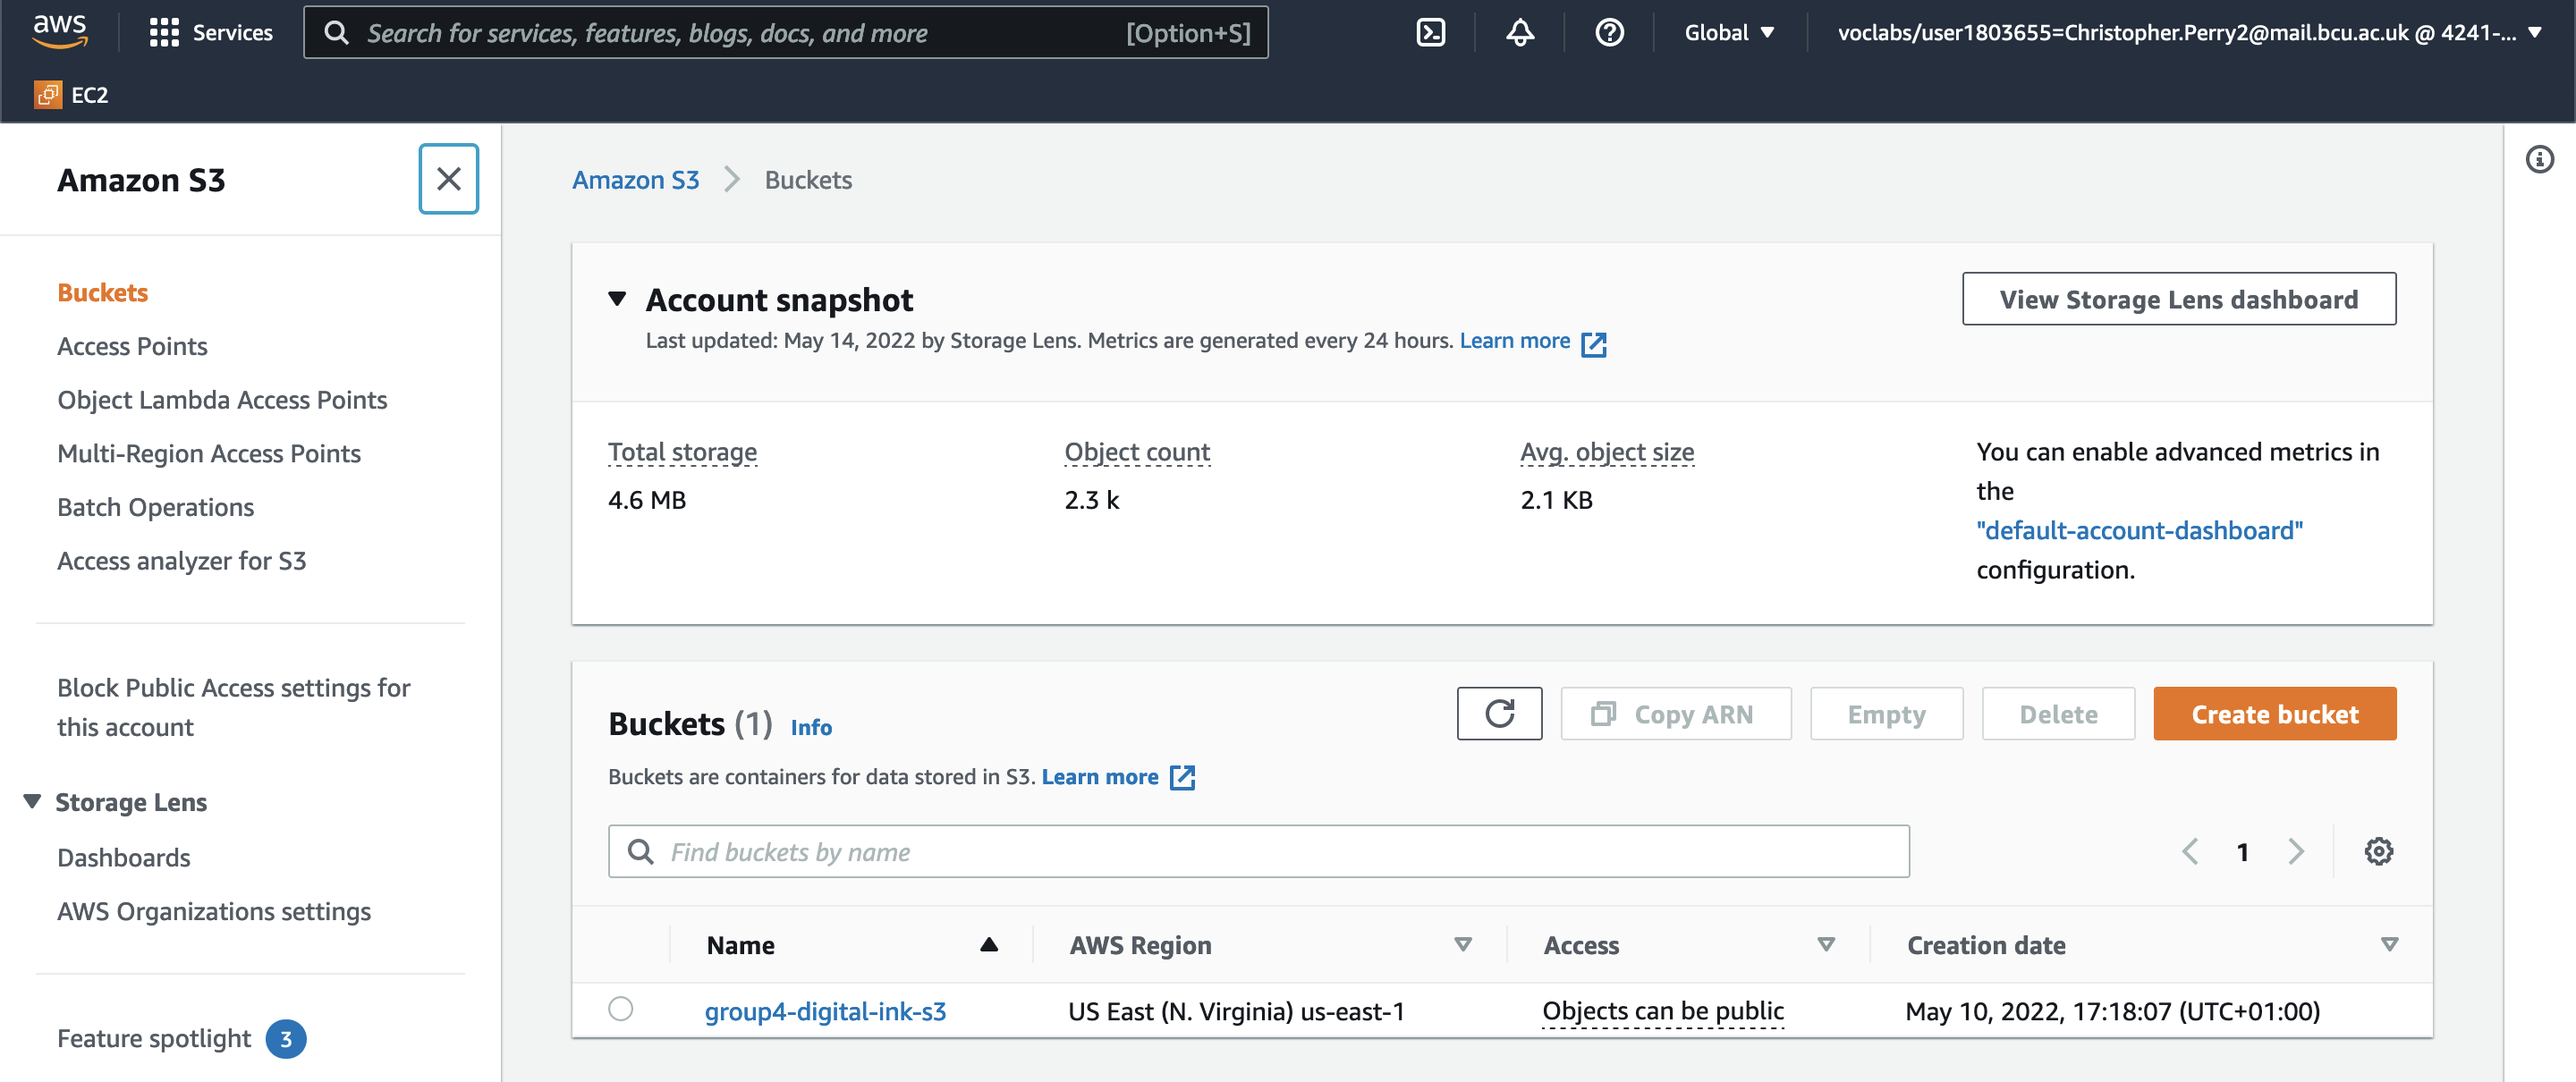
\includegraphics[width=\textwidth]{resources/s3/s3-created.png}
            \caption{S3 Bucket Successfully Created}
            \label{fig:s3-created}
        \end{figure}


    \section{Using S3 URLs within Code}


    \item Now that S3 bucket has been created, images must be uploaded.
        \begin{figure}[H]
            \centering
            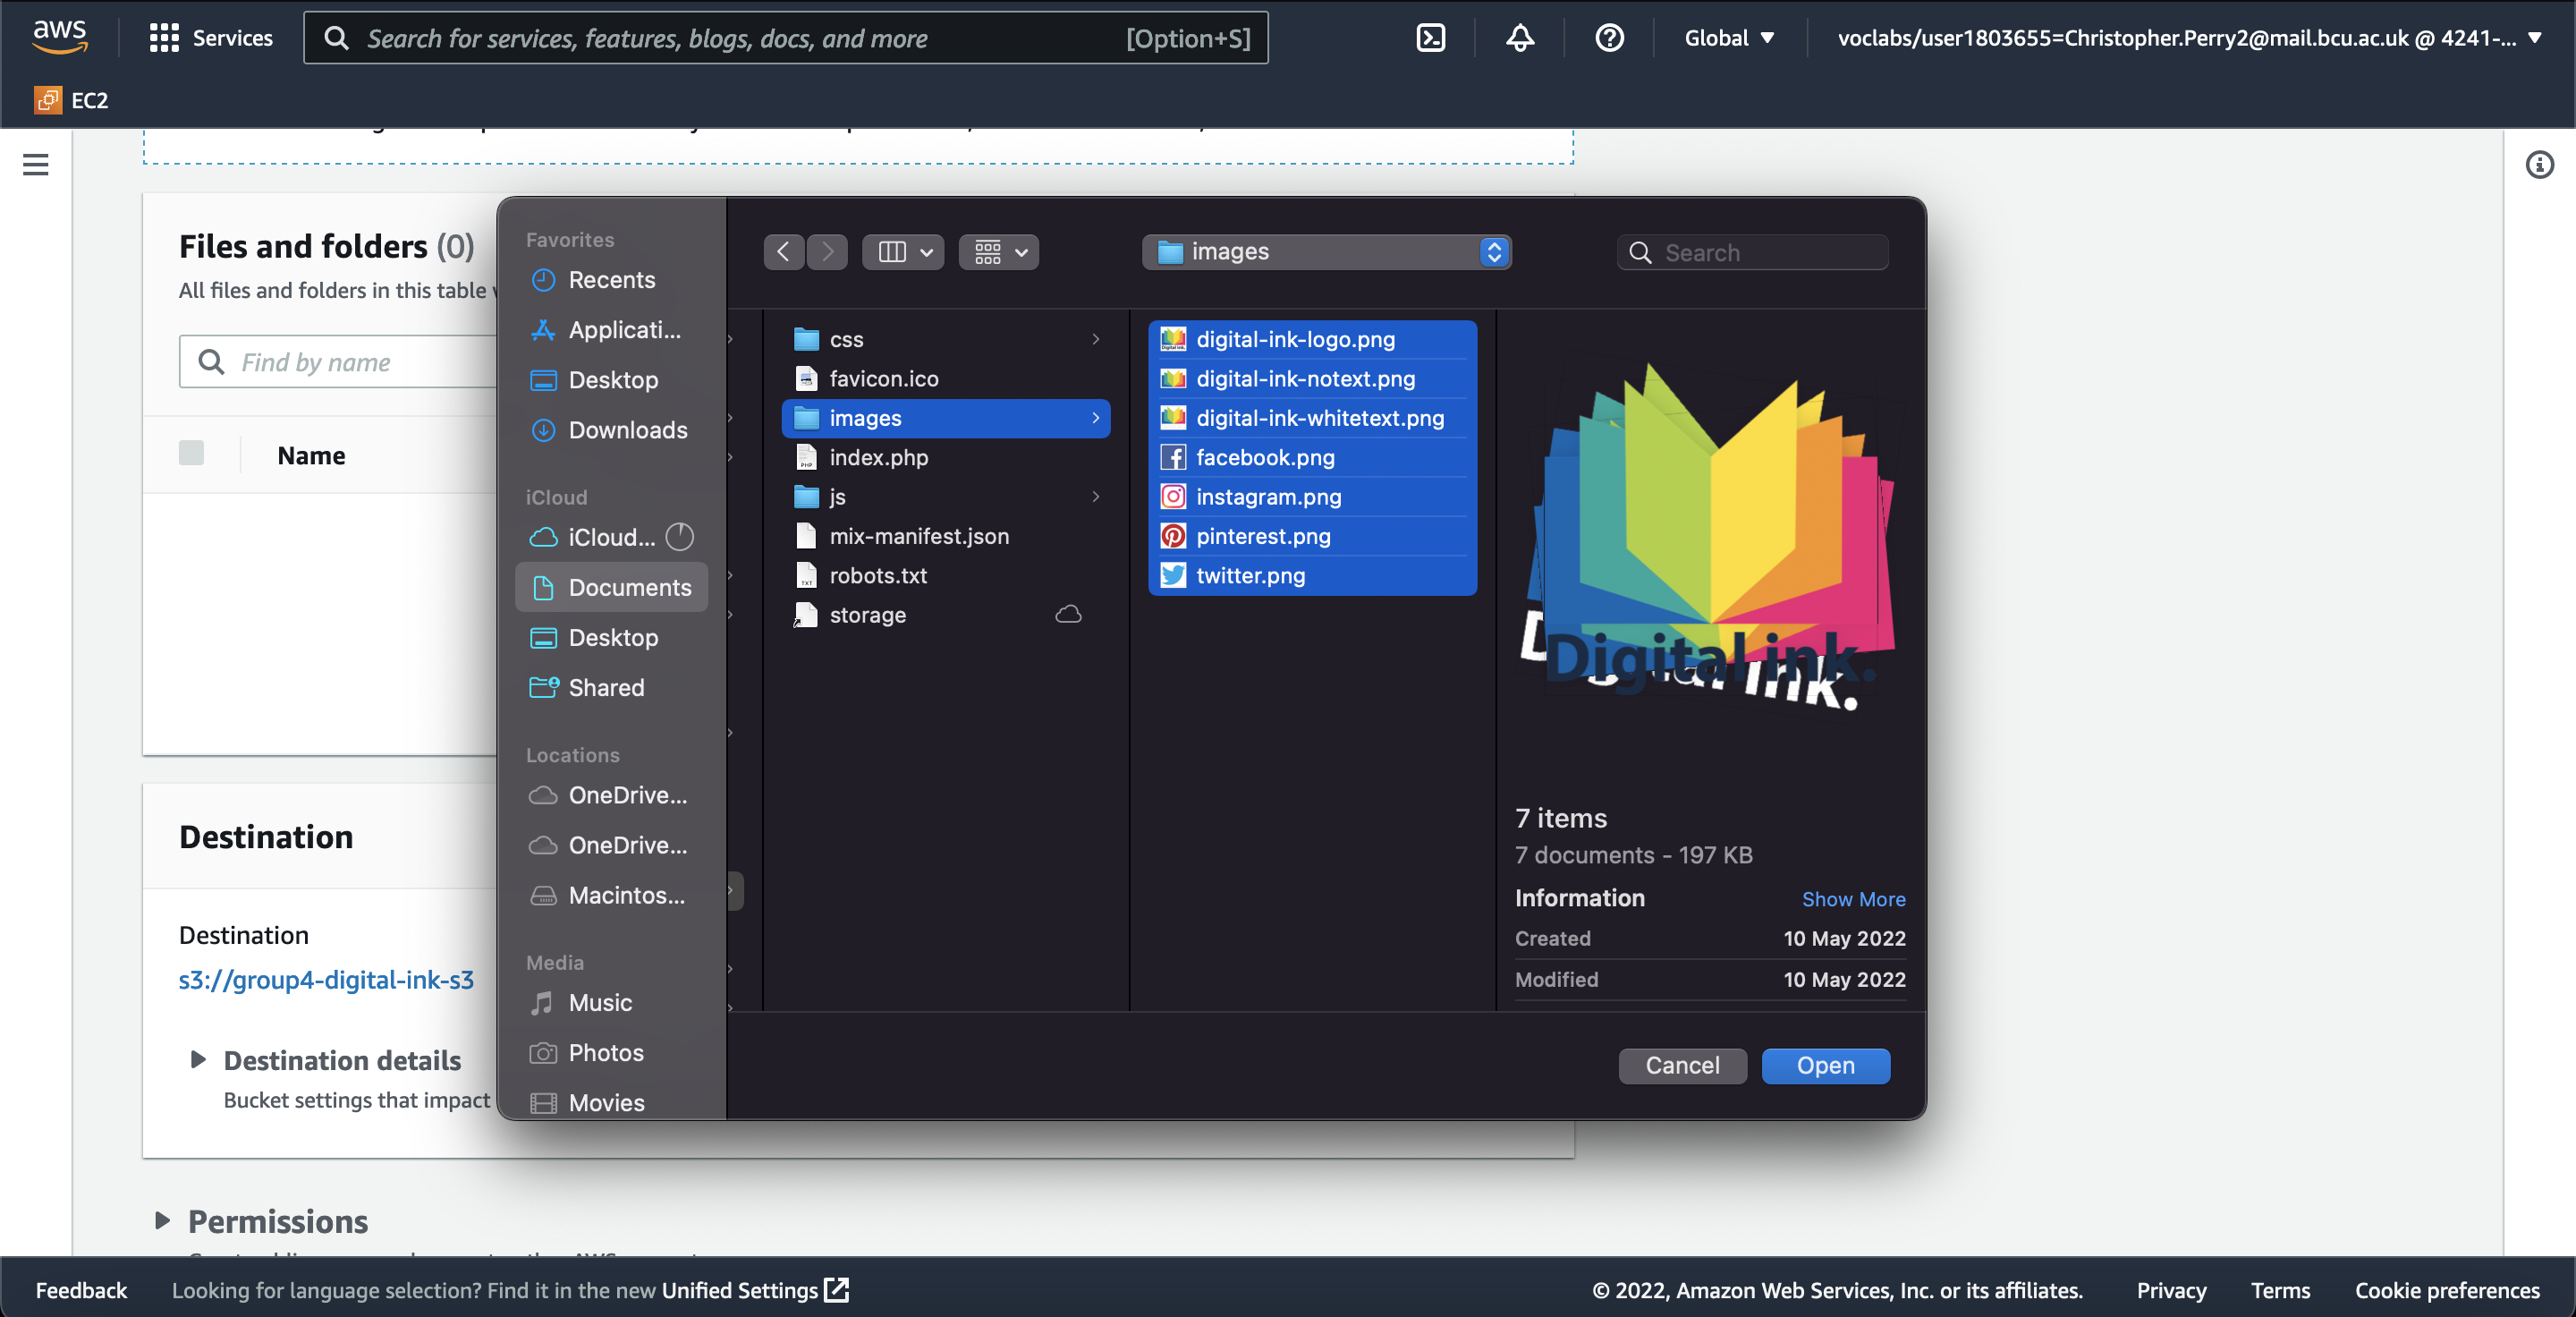
\includegraphics[width=\textwidth]{resources/s3/s3-image-upload.png}
            \caption{Uploading Static Assets to S3 Bucket}
            \label{fig:s3-image-upload}
        \end{figure}


    \item Double-check the upload summary to ensure only the correct images will be uploaded.
        \begin{figure}[H]
            \centering
            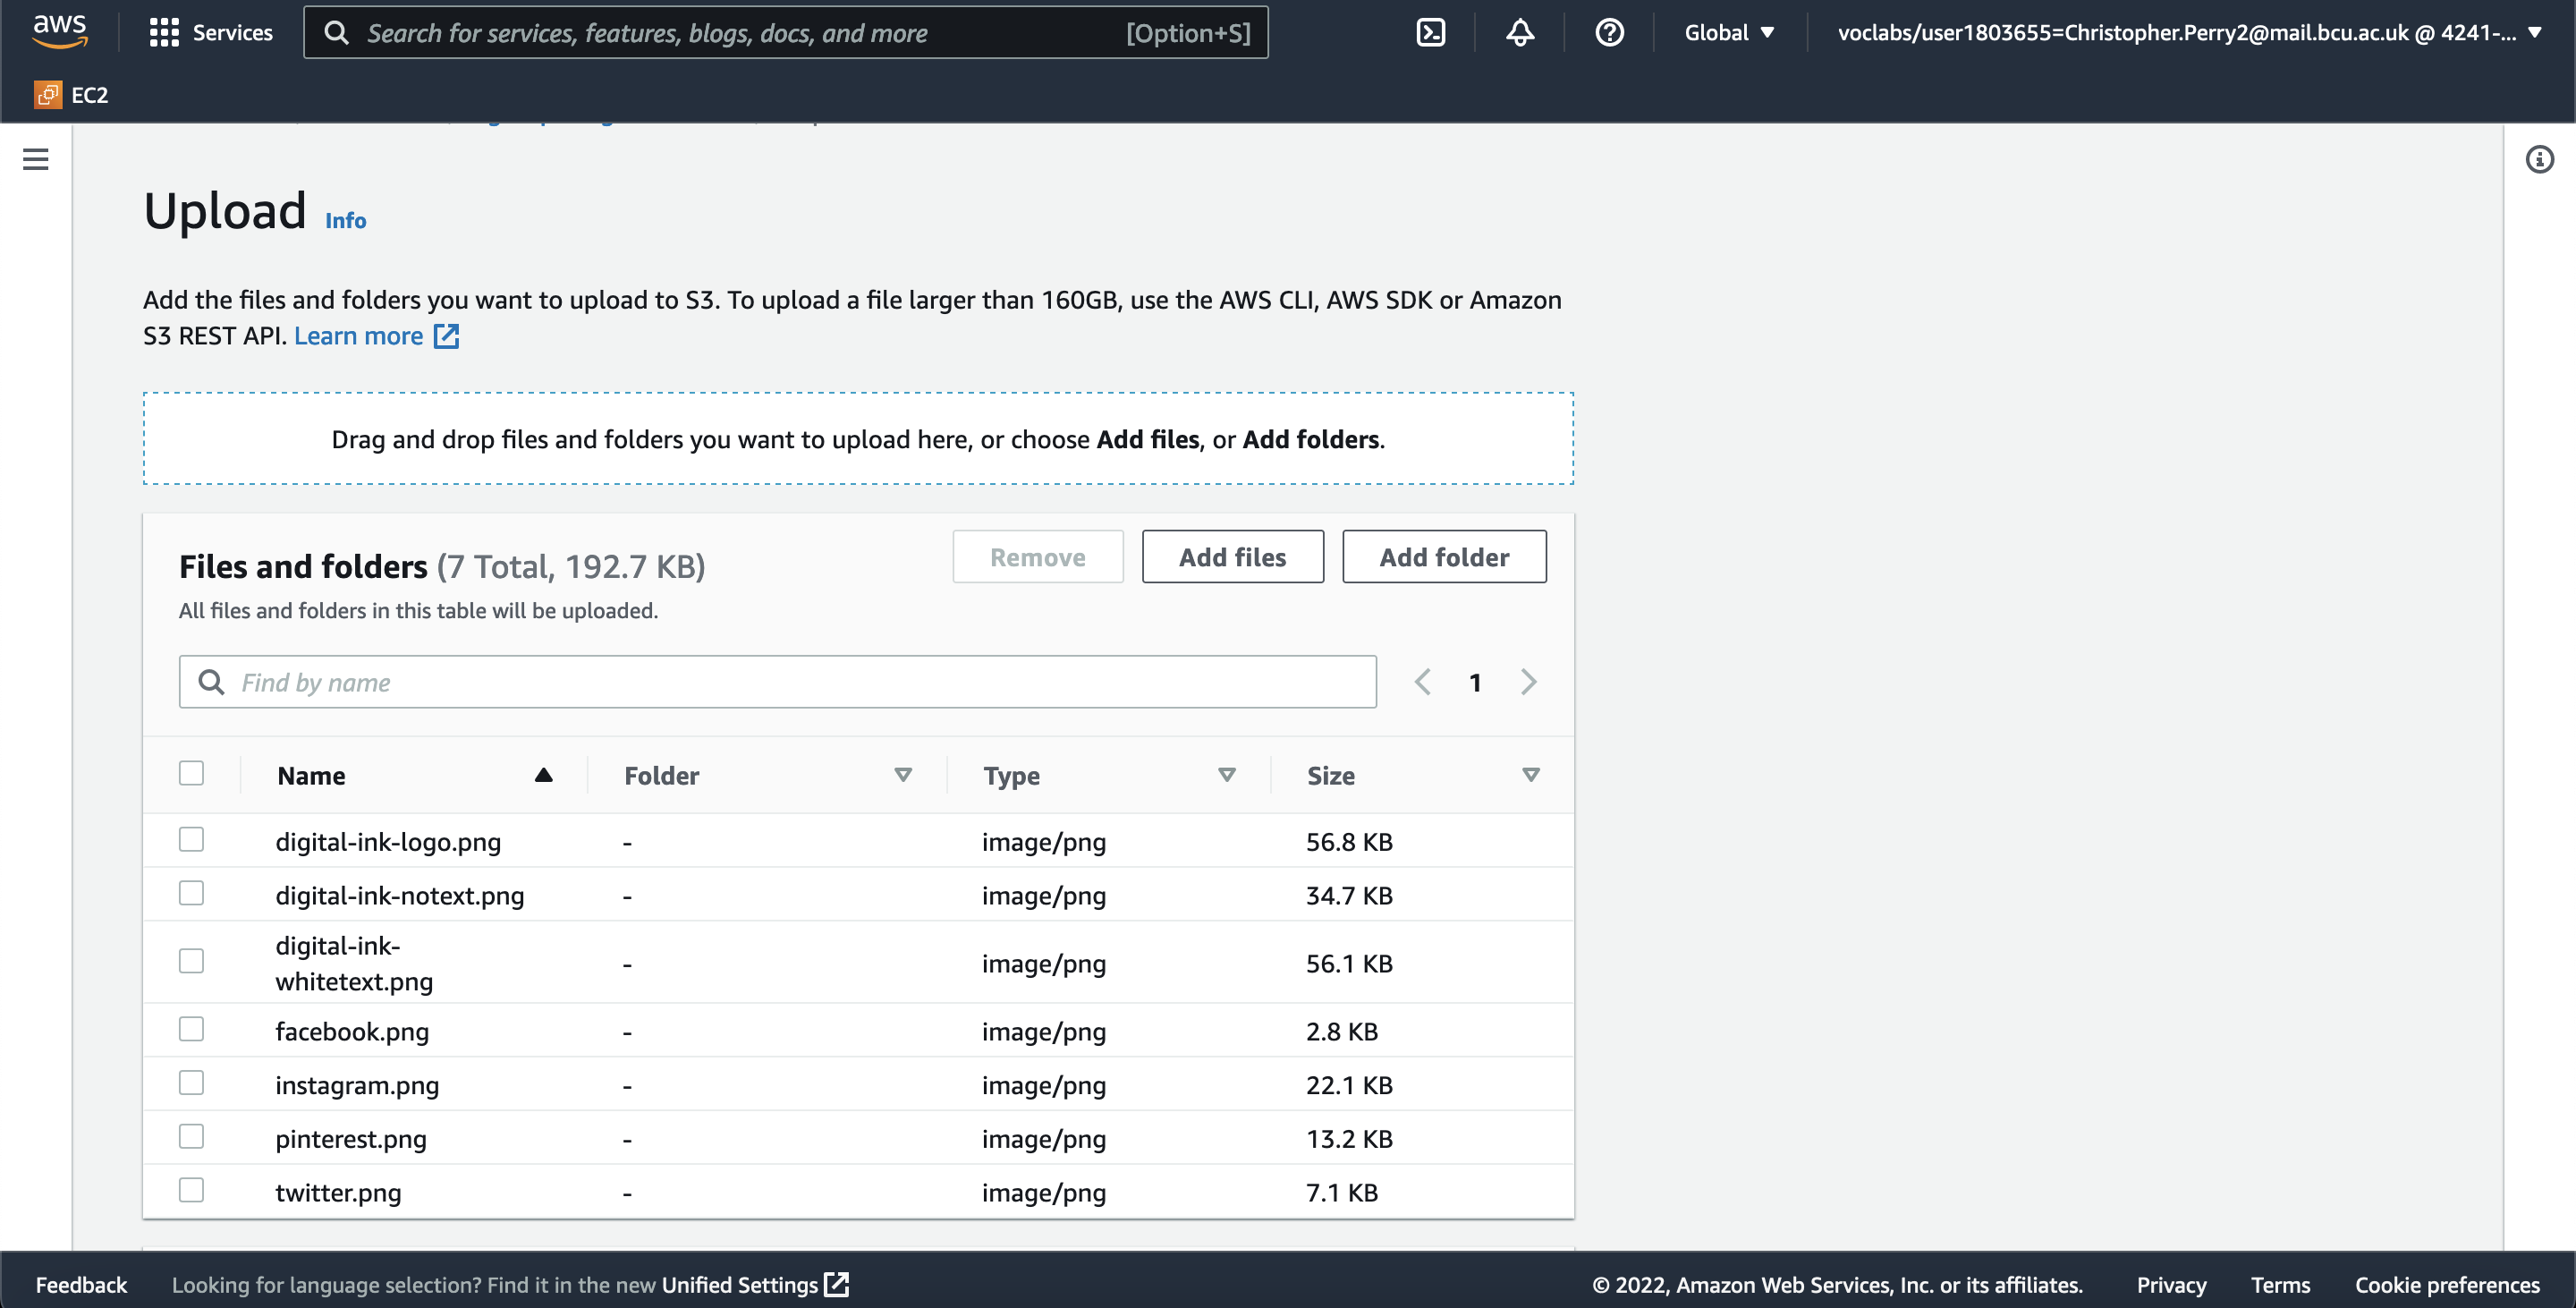
\includegraphics[width=\textwidth]{resources/s3/s3-upload-summary.png}
            \caption{Uploading all Static Assets to S3 Bucket}
            \label{fig:s3-upload-summary}
        \end{figure}

    \item Wait for images to upload.
        \begin{figure}[H]
            \centering
            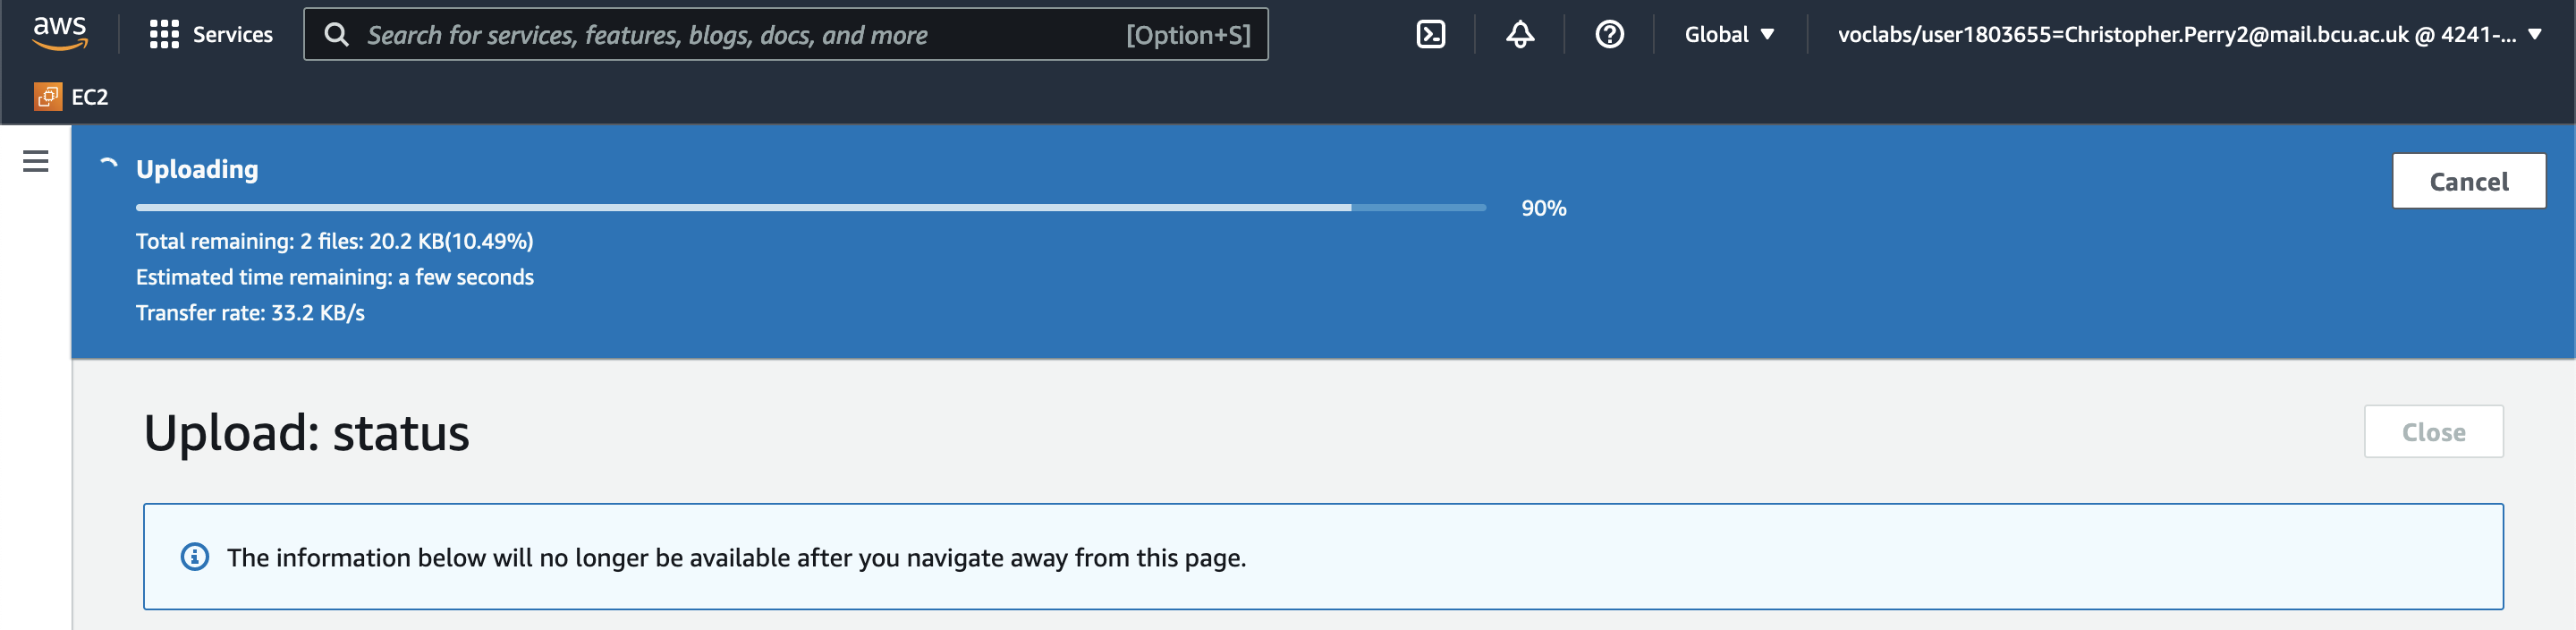
\includegraphics[width=\textwidth]{resources/s3/s3-uploading.png}
            \caption{S3 Uploading in Progress}
            \label{fig:s3-uploading}
        \end{figure}

    \item If successful, message shows indicating success.
        \begin{figure}[H]
            \centering
            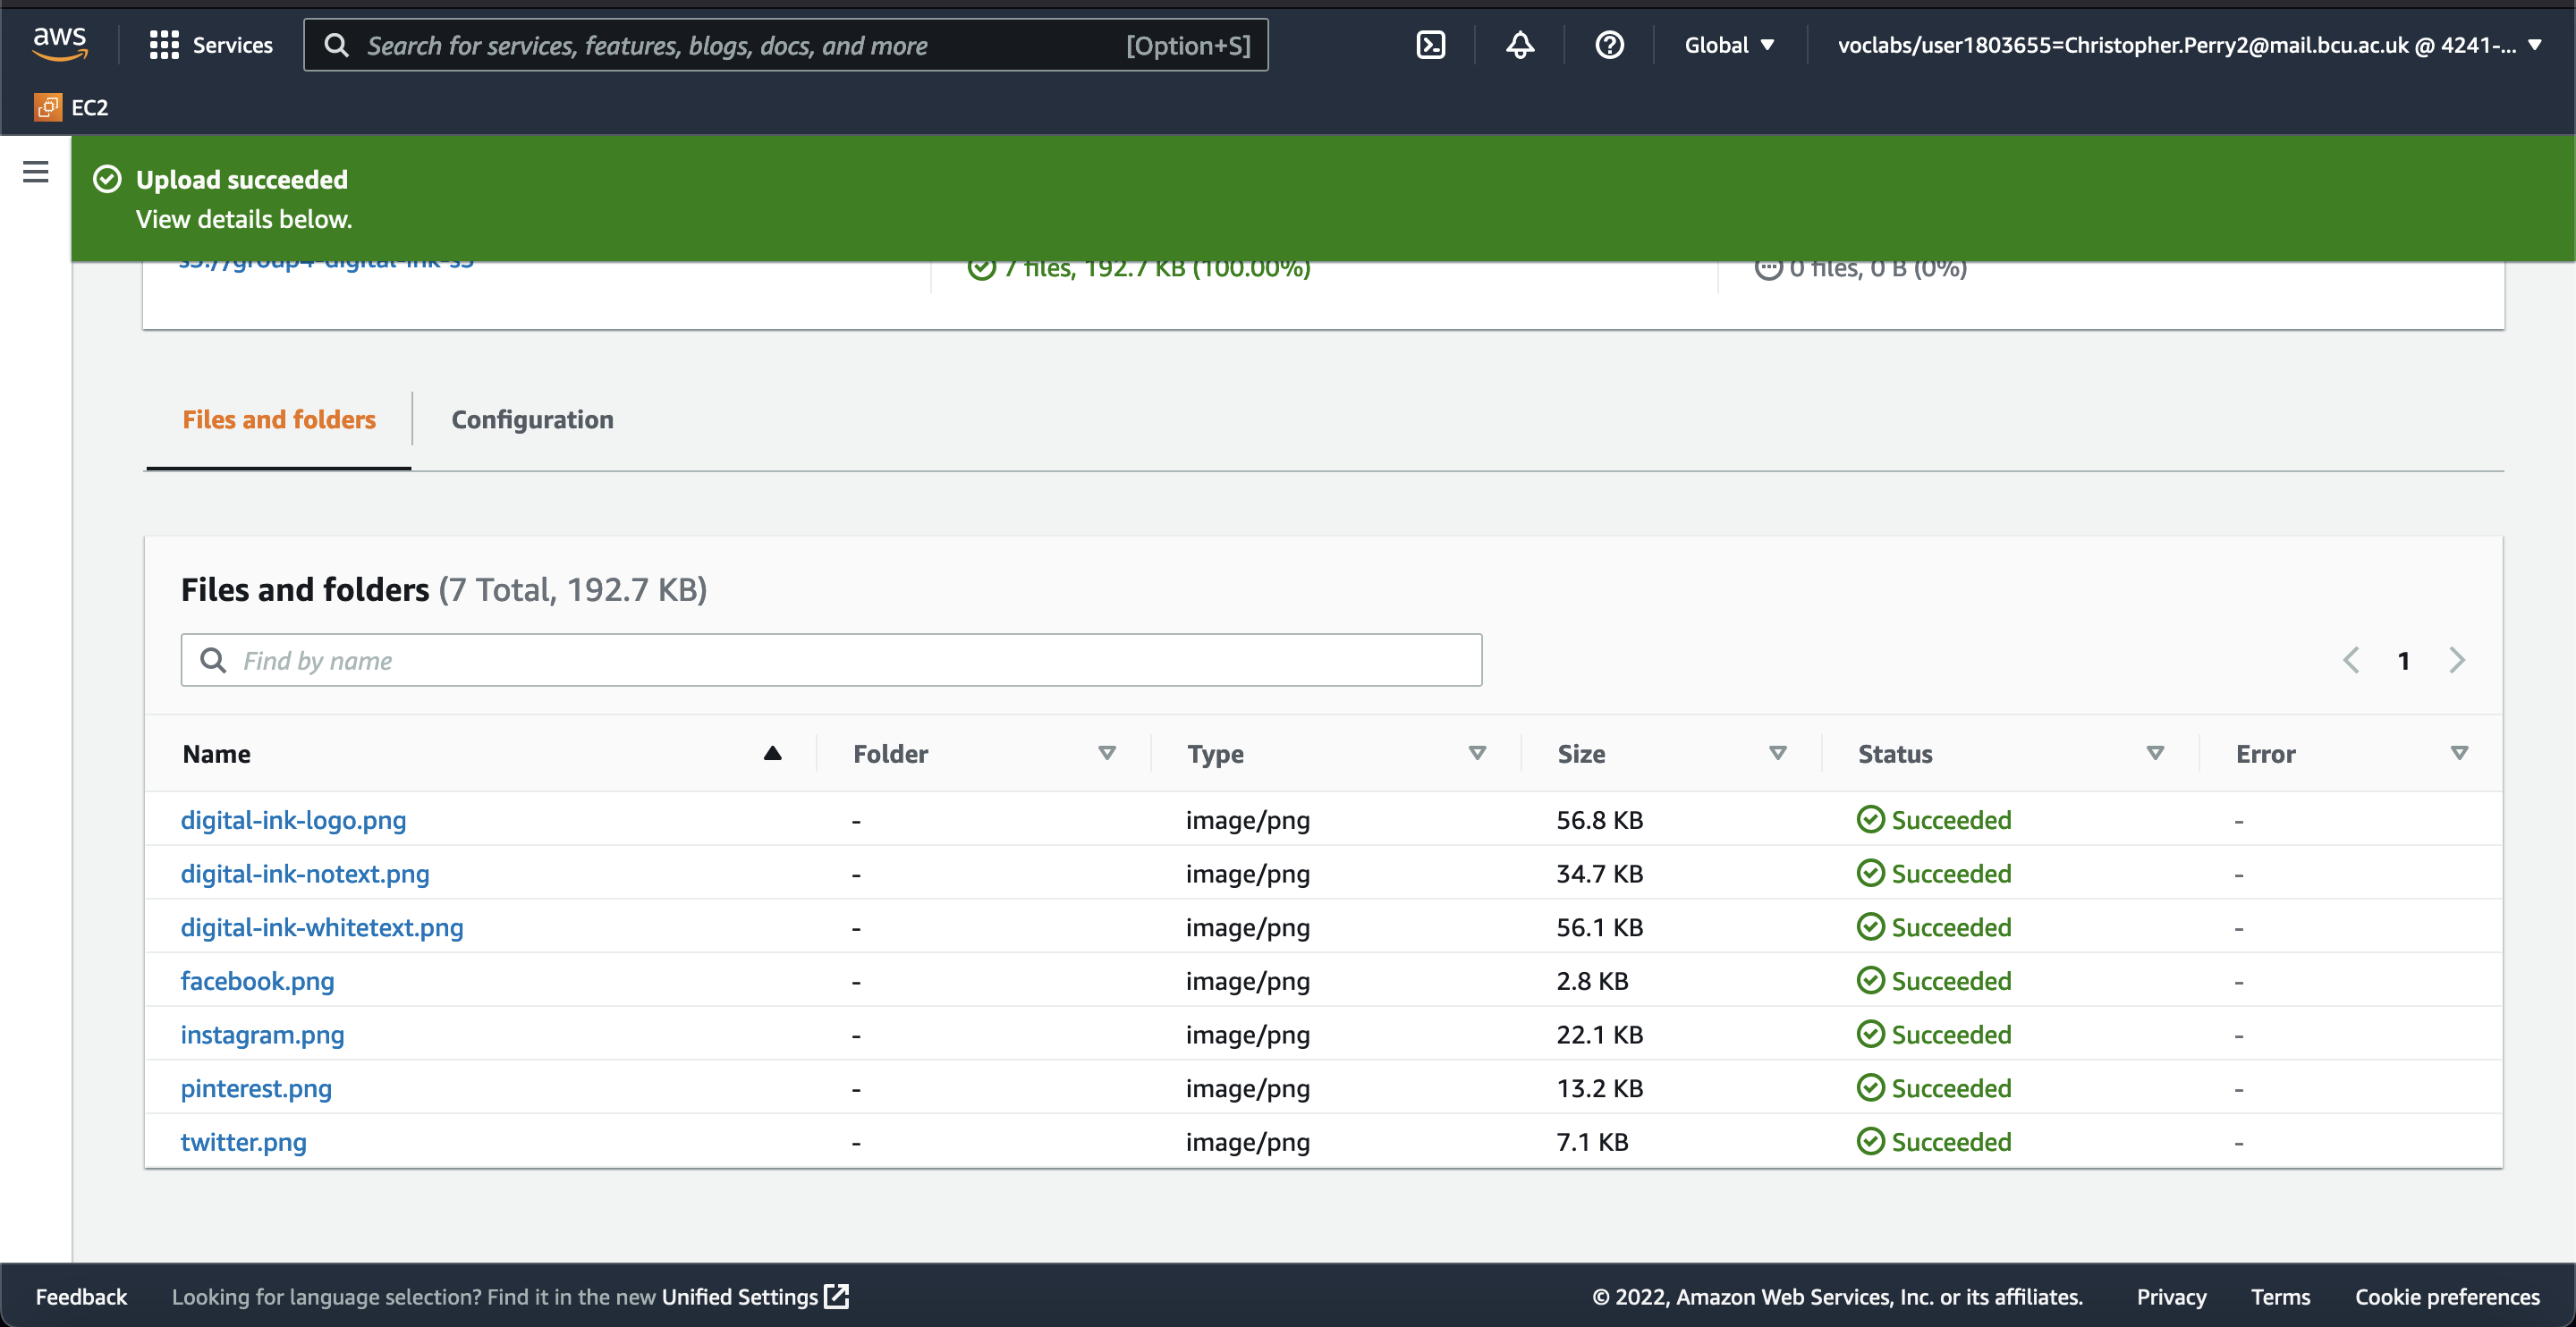
\includegraphics[width=\textwidth]{resources/s3/s3-uploaded.png}
            \caption{S3 Upload Success}
            \label{fig:s3-uploaded}
        \end{figure}

    \item Now that images have been uploaded, we must change the asset image paths in code to point to S3 instead of using local storage.
        \begin{figure}[H]
            \centering
            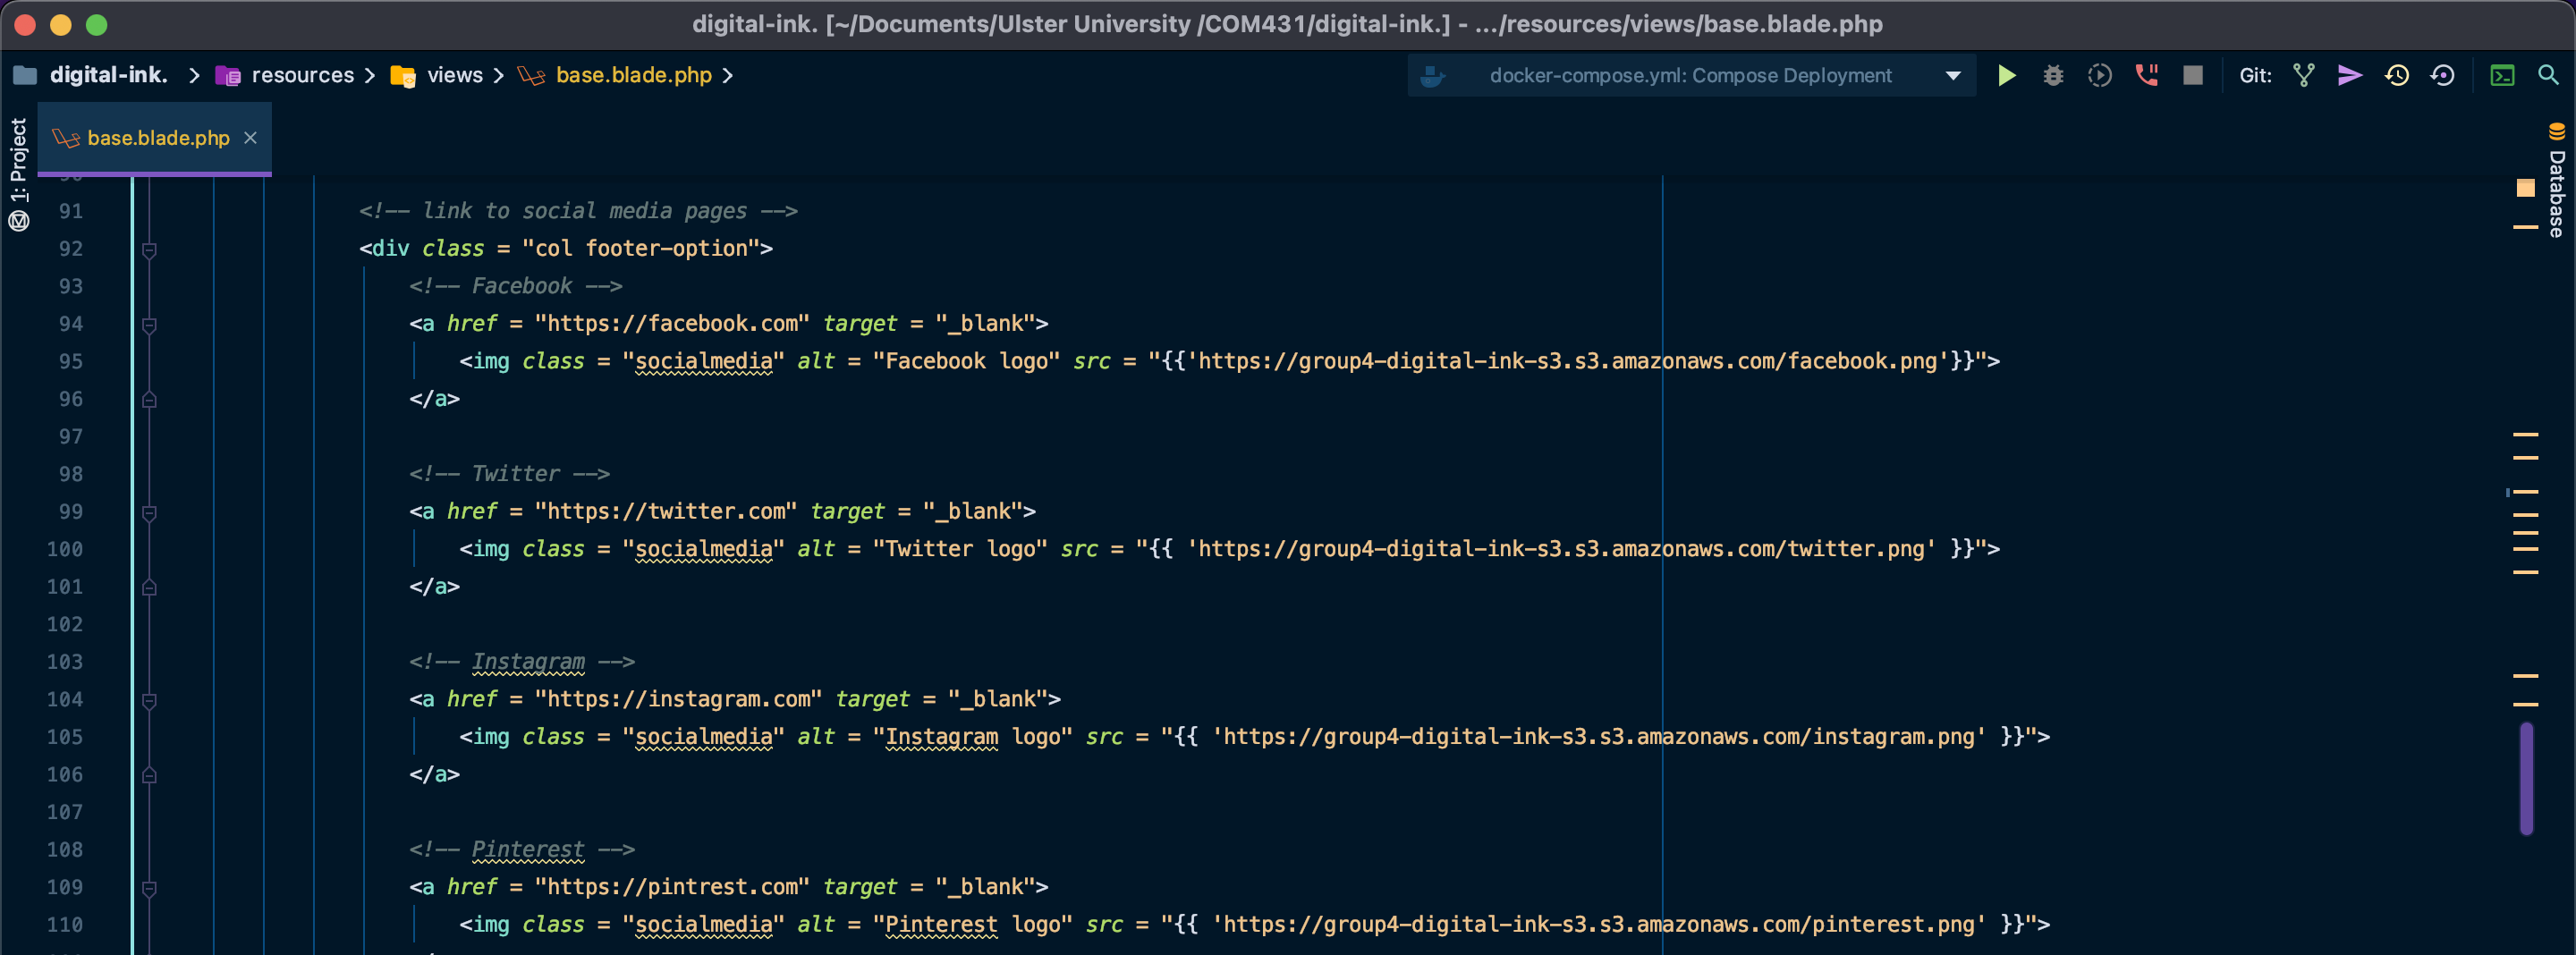
\includegraphics[width=\textwidth]{resources/s3/s3-url-change.png}
            \caption{Changing Image Paths within Code}
            \label{fig:s3-url-change}
        \end{figure}

    \section{Testing S3 Working}

    \item To test S3 is working, the URL may be visited in a browser for confirmation.
        \begin{figure}[H]
            \centering
            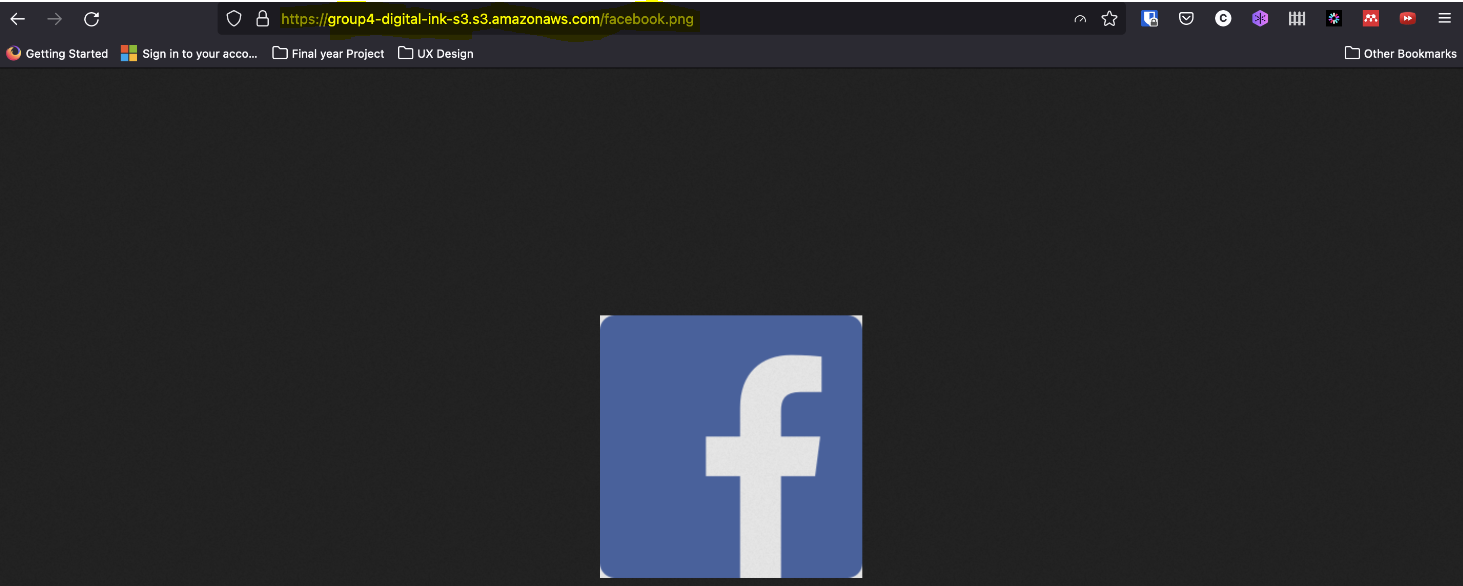
\includegraphics[width=\textwidth]{resources/s3/s3-image-displayed.png}
            \caption{Image access through S3}
            \label{fig:s3-image}
        \end{figure}


    \item Ensure that S3 billing is not too high, which will depend on how many GiB of images are uploaded.
        \begin{figure}[H]
            \centering
            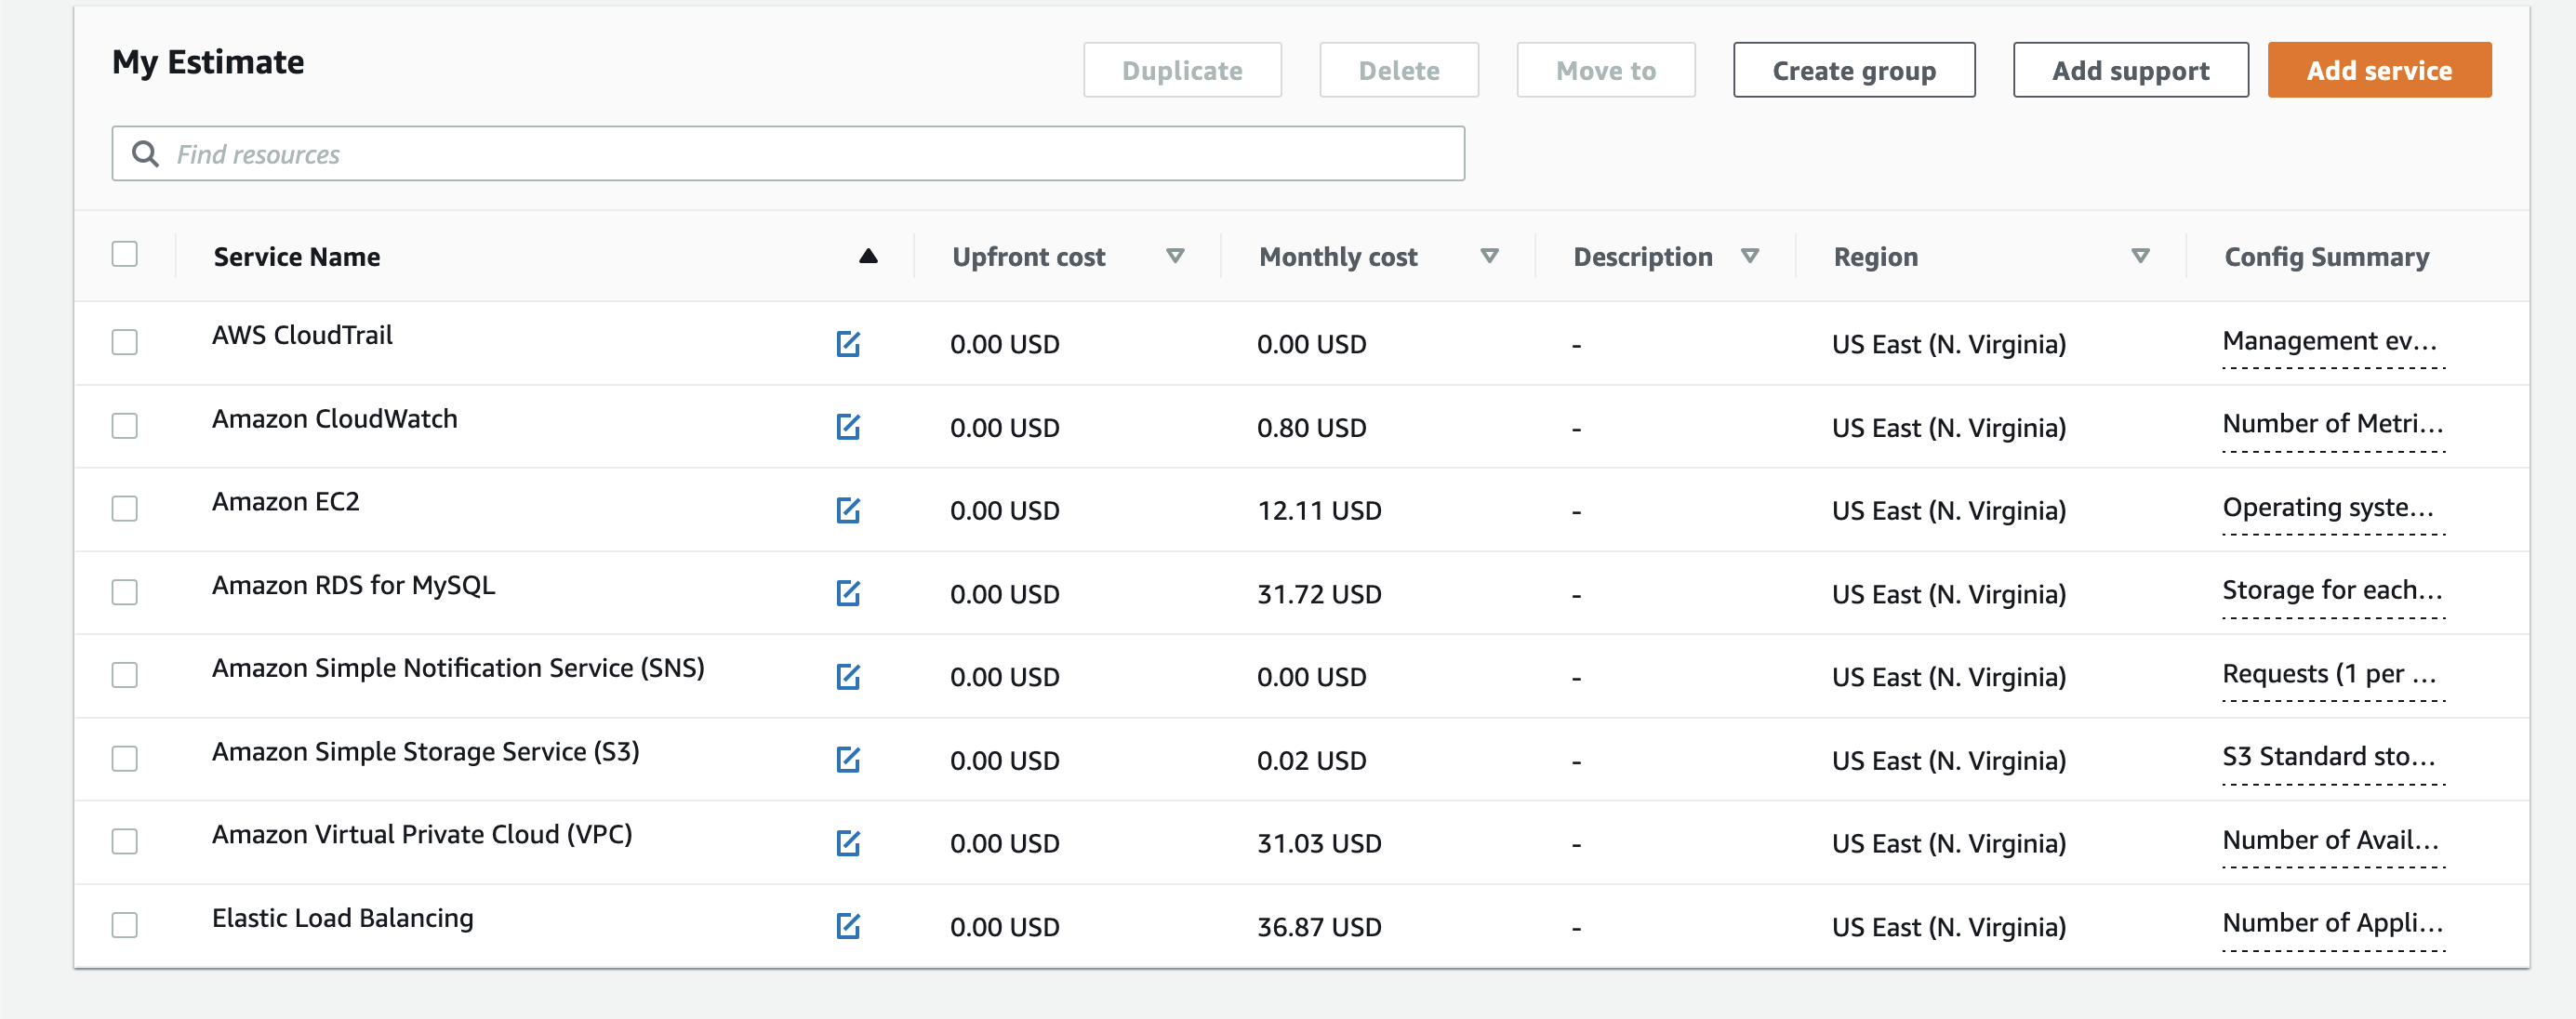
\includegraphics[width=\textwidth]{resources/s3/Screenshot 2022-05-14 at 6.45.18 pm.png}
            \caption{Billing Estimate for S3 Services}
            \label{fig:s3-billing}
        \end{figure}
\end{enumerate}

\section{Content Distribution Network (CDN)}
For adding a content distribution network to our S3 bucket, please see Chapter~\ref{ch:cloudfront}.

